\chapter{Non imaging optics}
This chapter provides some basic notions of illumination optics needed in this thesis.
\section{Radiometric and photometric variables}

\indent The radiant flux $\Phi_{\textrm{r}}$ (unit watt, [\textrm{W}]) is the total energy emitted from a source or received by a target per unit time:
\begin{equation}
\Phi_{\textrm{r}} = \frac{\textrm{d}Q}{\textrm{d}T}\,,
\end{equation}
where $Q$ is the energy and $T$ the time.\\
\indent The photometric variables differ from their radiometric counterparts in the sense that they only take into account the part of the spectrum perceived by the human eye as light.
 Therefore, the luminous flux $\Phi$ (unit lumen, [\textrm{lm}]) is defined as the perceived power of light by the human eye, \cite{chaves2015introduction}.
 These radiant and the luminous flux are related by the luminous efficacy function, unit [lm/W], that tells us how many lumen there are for each Watt of power at a given wavelength.
 The luminous efficacy reaches its maximum  at a wavelength of $555$ $\textrm{nm}$ where it is equal to $683$ $\textrm{lm}/\textrm{W}$.
  We may normalize the luminous efficacy function with its maximum value of $683$.
  This normalized function is the dimensionless luminosity function $\bar{y}(\lambda)$ shown in Figure $\ref{fig:luminosityfunction}$ where $\lambda$ is the wavelength.
\begin{figure}[htbp]
%\label{fig:luminousfunction}
  \begin{center}
  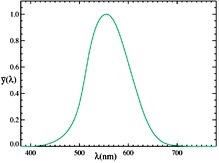
\includegraphics[width=7cm]{Luminosity}
  \end{center}
  \caption{Luminosity function $\bar{y}(\lambda)$: relation between the eye's sensitivity and the wavelength of the light. The luminous function is dimensionless.}
  \label{fig:luminosityfunction}
  \end{figure}
\\ The luminous flux corresponding to one Watt of radiation power at any wavelength is given by the product of $683$ $\textrm{lm/W}$ and the luminosity function at the same wavelength,
i.e. $683 \, \bar{y}(\lambda)$. Hence, $\Phi$ has unit lumen [\textrm{lm}] and it is defined as:
\begin{equation}
\Phi = 683 \int_0^\infty \Phi_\textrm{r}(\lambda) \bar{y}(\lambda)\textrm{d}\lambda \;.
\end{equation}
Therefore the units of the luminous flux are: $$[\textrm{lm/W}]\,[ \textrm{W}] = [\textrm{lm}]. $$
\indent The luminous flux $\textrm{d}\Phi$ falling on a surface is called illuminance $E$ \big(unit \big[$\textrm{lm}/\textrm{m}^2\big]$\big)
and is defined as:
\begin{equation}
 E=\frac{\textrm{d}\Phi}{\textrm{d}A}\;,
 \end{equation}
 where $\textrm{d}A$ is an infinitesimal area receiving energy.
 Hence the illuminance is only defined at the target.
The luminous intensity $I$ (unit candela (\textrm{cd}), $[\textrm{cd}=\textrm{lm}/\textrm{sr}]$) is defined as the luminous flux $\textrm{d}\Phi$ per solid angle
$\textrm{d}\Omega$ and is given by:
\begin{equation}\label{intensity}
I = \frac{\textrm{d}\Phi}{\textrm{d}\Omega}\;.
\end{equation}
 \begin{figure}[htbp]
%\label{fig:cup}
  \begin{center}
  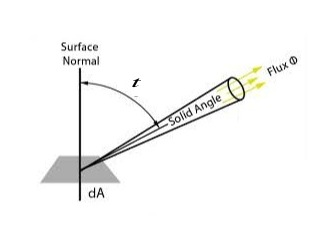
\includegraphics[width=6 cm]{radiation}
  \end{center}
  \caption{Radiation emitted in a solid angle $\textrm{d}\Omega$ in a direction making an angle $t$ with the normal to the area $\textrm{d}A$.}
  \label{fig:rad}
  \end{figure}
The luminance $L$ \big(unit $\big[\textrm{cd} / \textrm{m}^2\big]$\big) is the luminous flux per unit area $\cos(t)\,\textrm{d}A$ perpendicular to the ray and per unit solid angle $\textrm{d}\Omega$
and it is given by:
\begin{equation}\label{luminance1}
  L=\frac{\textrm{d}^2\Phi}{\cos t\textrm{d}A\textrm{d}\Omega}\;,
\end{equation}
where $t$ is the angle that the normal to area $\textrm{d}A$ makes with the direction of the solid angle $\textrm{d}\Omega$, as shown in Figure $\ref{fig:rad}$.
\noindent Note that from ($\ref{intensity}$) and ($\ref{luminance1}$) we can derive a relation between the intensity and the luminance.\\
The elementary intensity emitted by an elementary area $\textrm{d}A$ is given by:
\begin{equation}
\textrm{d}I = \frac{\textrm{d}\Phi}{\textrm{d}\Omega}= L(\textrm{x},t)\cos(t)\textrm{d}A \,,,
\end{equation}
where $\cos(t) \textrm{d}A$ is the projection of the area element $\textrm{d}A$ on a line perpendicular to the ray.
When the luminance is uniform over a finite area $A$, the luminous intensity emitted in the direction $t$ is equal to:
\begin{equation}
I(t) = L A \cos(t)\,.
\end{equation}
Thus, when $L(\textrm{x},t)$ does not depend on the position and the direction (i.e. $L(\textrm{x},t)=L$), we deduce Lambert's cosine law:
\begin{equation}
I(t) = I_0\cos(t)\,.
\end{equation}
\indent In this thesis we consider two-dimensional optical systems. 
 Hence, we need to find two-dimensional analogies for the definitions given above.
In two dimensions the illuminance \big(unit $\big[\textrm{lm}/\textrm{m}\big]$\big) denotes the luminous flux falling on a line segment $\textrm{d}x$ and is given by:
 \begin{equation}
 E=\frac{\textrm{d}\Phi}{\textrm{d}x}\;.
 \end{equation}
 The luminous intensity \big(unit $\big[\textrm{lm}/\textrm{rad}\big]$\big) is the luminous flux per angle $\textrm{d}t$:
 \begin{equation}
 I=\frac{\textrm{d}\Phi}{\textrm{d}t}\;.
 \end{equation}
 Thus the following relation holds:
 \begin{equation}
 \textrm{d}I = L\cos(t)\textrm{d}x\,.
 \end{equation}
 Finally, the luminance \big(unit $\big[\textrm{lm}/(\textrm{rad}\; \textrm{m})\big]$\big) is given by:
 \begin{equation}
 L = \frac{\textrm {d}^2 \Phi}{\cos t\,\textrm{d}x \,\textrm{d}t}.
 \end{equation}
 \indent In a homogeneous medium the luminance is conserved along a ray.
%It is important to recall the conservation property of the luminance along rays.
Consider a light ray emitted from a segment with infinitesimal length $\textrm{d}a_1$ that hits an infinitesimal segment $\textrm{d}a_2$. %as presented in Figure
We suppose that the line segments are located at a distance $r$, see Figure $\ref{fig:grafico}$. The flux passing though $\textrm{d}a_2$ coming from $\textrm{d}a_1$ is equal to:
\begin{equation}
\textrm{d}\Phi_1 = L_1 \cos(t_1) \textrm{d}a_1 \textrm{d}t_1
\end{equation}
with \begin{equation}
\textrm{d}t_1 = \frac{\textrm{d}a_2\cos(t_2)}{r}
\end{equation}
and
\begin{equation}
\textrm{d}t_2 = \frac{\textrm{d}a_1\cos(t_1)}{r}\,.
\end{equation}
Let us consider the quantity
\begin{equation}\label{etendue}
\textrm{d}U = n \cos(t)\textrm{d}a\textrm{d}t= \textrm{d}a\textrm{d}(\tau).
\end{equation}
The quantity $U$ (unit $[m\; rad]$) is called \'{e}tendue and it characterizes the ability of an optical system to accept light. The \'{e}tendue is a measure of the flux gathering capability of the optical system, it is also called throughput of the optical system.\\
Then \begin{equation}
\label{etendue1}
\textrm{d}U_1 = n \textrm{d}a_1\cos(t_1)\textrm{d}t_1= \frac{n \textrm{d}a_1\cos(t_1)\textrm{d}a_2\cos(t_2)}{r},
\end{equation}
and
\begin{equation}
\label{etendue2}
\textrm{d}U_2 = n \textrm{d}a_2\cos(t_2)\textrm{d}t_2= \frac{ n \textrm{d}a_2\cos(t_2)\textrm{d}a_1\cos(t_2)}{r}\,.
\end{equation}
From equation ($\ref{etendue1}$) and ($\ref{etendue2}$) we see that $\textrm{d}U_1=\textrm{d}U_2$.
For a light beam, all the light passing through $\textrm{d}a_1$ coincides with the light passing through $\textrm{d}a_2$, hence $\textrm{d}U = \textrm{d}U_1$. Moreover, for the same light beam, all the light passing from $\textrm{d}a_2$ corresponds to the light emitted from $\textrm{d}a_1$, then $\textrm{d}U=\textrm{d}U_2$. Finally we can conclude that the \'{e}tendue $\textrm{d}U$ is conserved along a beam of light. Since also the flux through the areas $\textrm{d}a_1$ and $\textrm{d}a_2$ is conserved, the following relation holds:
\begin{equation}\label{basicluminance}
L := n \frac{\textrm{d}\Phi}{\textrm{d}U} = constant\,.
\end{equation}
The previous relation is also valid when the light propagates through two media with different refractive indexes. In that case both the luminance $L$ and the basic luminance $L^*:= L/n$ are conserved with $n$ the refractive index of the medium. In the optical systems we will consider in this work, the source and the target are located in the same media (air) with $n=1$, so the luminance and the basic luminance are equal at the source and the target of the system.\\
\begin{figure}[htbp]
 \label{fig:grafico}
     \begin{center}
     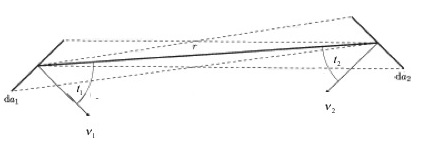
\includegraphics[width=10cm]{grafico.jpg}
     \end{center}
     \caption{\footnotesize{$\textrm{d}a_1$ and $\textrm{d}a_2$ are two line segments with normal $\nu_1$ and $\nu_2$, respectively, that make an angle $t_1$ and $t_2$ with the central ray.}}
\label{fig:rays}
 \end{figure}

\section{Reflection and refraction law}
The propagation of a light ray traveling through  different media is described by the reflection and refraction law.
In this section we introduce these two laws and we explain the total internal reflection phenomenon.
A light ray is described by a position vector \vect{x} and a direction vector \vect{t} and can be parameterized by the arc length \variabileiabileiabile{s}.
Light rays travel in an homogeneous medium along straight lines, once they hit a reflective surfaces their direction changes.
 Denoting with $\vect{t}_1$ the direction of the incident ray and with $\boldsymbol{\nu}$ the unit normal to the surface at the location of the incidence, the direction $\vect{t}_2$ of the reflected ray is given by:
 \begin{equation}\label{Reflection}
  \vect{t}_2 = \vect{t}_1-2(\vect{t}_1,\boldsymbol{\nu})\boldsymbol{\nu}\,,
\end{equation}
where the vectors $\vect{t}_1$ and $\boldsymbol{\nu}$ are unit vectors. 
From Eq. (\ref{Reflection}) it follows that the vector  $\vect{t}_2$ is a unit vector too, indeed considering the scalar product $(\vect{t}_2,\vect{t}_1)$ it holds:
\begin{equation}\label{unit_vector}
(\vect{t}_2,\vect{t}_1) = (\vect{t}_1,\vect{t}_1) - 4(\vect{t}_1,\boldsymbol{\nu})(\vect{t}_1,\boldsymbol{\nu})+
4(\vect{t}_1,\boldsymbol{\nu})^2(\boldsymbol{\nu},\boldsymbol{\nu})=1 .
\end{equation} 
The reflection law states that the incident angle $\alpha_\textrm{i}$ is equal to the reflective angle $\alpha_\textrm{r}$ which are measured counterclockwise with respect to the normal $\boldsymbol{\nu}$ of the surface, see Fig. \ref{Snell}.
When a ray propagates through two media with two different indices of refraction, $n_1$ and $n_2$, the direction of the refractive ray is given by:
\begin{equation}\label{Refraction}
\vect{t}_2 = n_{1,2}\,\vect{t}_1+
\Big[\sqrt{1-n_{1,2}^2+n_{1,2}^2(\boldsymbol{\nu},\vect{t}_1)^2}-n_{1,2}(\boldsymbol{\nu},\vect{t}_1) \Big]\boldsymbol{\nu}\,,
\end{equation}
where $n_{1,2}=n_1/n_2$. \\
 \indent Note that in Eq. (\ref{Reflection}) the direction of the normal $\boldsymbol{\nu}$ to the surface is not relevant for the computation of the direction of the reflective ray, since:
\begin{equation}
\vect{t}_2 = \vect{t}_1-2(\vect{t}_1,\boldsymbol{\nu})\boldsymbol{\nu}= \vect{t}_1-2(\vect{t}_1,-\boldsymbol{\nu})(-\boldsymbol{\nu}) ,
\end{equation}
while this is not the case of Eq. (\ref{Refraction}), therefore in the latter case we need to specify the direction of the vector $\boldsymbol{\nu}$ which is chosen in such a way that the angle that it forms with the incident ray $\vect{t}_1$ is smaller than or equal to $\pi/2$. Hence, if $(\vect{t}_1, \boldsymbol{\nu})\geq0$ the normal $\boldsymbol{\nu}$ directed inside the same medium in which travels the incident ray is taken, otherwise the normal $-\boldsymbol{\nu}$ directed inside the same medium in which the transmitted ray will travel has to be considered. \\ \indent
Eq. (\ref{Refraction}) is only valid for 
\begin{equation}\label{tir}\begin{split}
1-n_{1,2}^2+n_{1,2}^2(\boldsymbol{\nu},\vect{t}_1)^2\geq 0 & \Rightarrow \frac{n_2}{n_1}\geq \sqrt{1-(\boldsymbol{\nu},\vect{t}_1)^2}\\
\Rightarrow n_2\geq n_1\sqrt{1-\cos^2(\alpha_\textrm{i})} & \Rightarrow  n_2\geq n_1 \sin(\alpha_\textrm{i})
\end{split}
\end{equation}
\\ \indent
 The angle for which the equality holds is
\begin{equation}\label{critical}
\alpha_{\textrm{c}} = \arcsin\Big(\frac{n_2}{n_1}\Big)
\end{equation} and it is called the critical angle, \cite{chaves2015introduction}.
Note that the condition $\frac{n_2}{n_1}<1$ is verified as in this case $\sin(\alpha_\textrm{i})<1$.
When the incident angle $\alpha_{\textrm{i}}$ is exactly equal to the critical angle $\alpha_{\textrm{c}}$ the refractive ray propagates parallel to the refractive surface, 
when $\alpha_{\textrm{i}}>\alpha_{\textrm{c}}$ the light ray is no longer refracted but it is reflected by the surface. This phenomenon is called total internal reflection (TIR). 









































\section{Fresnel reflection}
%\section{Application to optical design systems}